\section{25 de enero de 2021}

\subsection{Topología de Espacios Métricos}
\begin{definition}
Sea $(M,d)$ un espacio métrico. 
\begin{enumerate}
    \item La \textbf{Bola abierta} de centro en $a$ y radio $r$ es: $B_r(a)\{x\in M\ni d(x,a)<r\}$
    \item La \textbf{Bola cerrada} de centro en $a$ y radio $r$ es $\Bar{B}_r(a)=B_r[a]=\{x\in M\ni d(x,a)\leq r\}$
\end{enumerate}
\end{definition}

\begin{remark}
\begin{enumerate}
    \item En el caso que $M=\mathbb{R}$ y $d(x,y)=|x-y|,\forall x,y\in\mathbb{R},\implies B_r(a)=\{x\in\mathbb{R}:|x-a|<r\} =\{x\in\mathbb{R}: a-r<x<a+r\}=(a-r,a+r)$. Que es análogo para $[a-r,a+r]$
    \item En el caso de $\mathbb{R}^2$ o $\mathbb{C}$, las bolas se llaman discos. 
    \item Un subconjunto de un espacio métrico es acotado si está contenido en una bola; $A\subset M$ es acotado, si $\exists r>0,a\in M\ni A\subset B_r (a)$. (i.e. $d(x,a)<r,\forall x\in A)$.
    \item Las bolas abiertas y cerradas son acotadas. 
\end{enumerate}
\end{remark}
\marginnote{Los elementos de una topología se le llama abiertos.}
\begin{definition}
\begin{enumerate}
    \item  Un subconjunto $u$ del espacio métrico $M$ es un abierto, si $\forall a\in u\exists r>0 \ni B_r(a)\subset u$
    \begin{center}
        

\tikzset{every picture/.style={line width=0.75pt}} %set default line width to 0.75pt        

\begin{tikzpicture}[x=0.75pt,y=0.75pt,yscale=-1,xscale=1]
%uncomment if require: \path (0,300); %set diagram left start at 0, and has height of 300

%Shape: Circle [id:dp5694297831696636] 
\draw  [dash pattern={on 4.5pt off 4.5pt}] (162,137.9) .. controls (162,84.38) and (205.38,41) .. (258.9,41) .. controls (312.42,41) and (355.8,84.38) .. (355.8,137.9) .. controls (355.8,191.42) and (312.42,234.8) .. (258.9,234.8) .. controls (205.38,234.8) and (162,191.42) .. (162,137.9) -- cycle ;
%Shape: Circle [id:dp0054591279969846696] 
\draw  [color={rgb, 255:red, 255; green, 0; blue, 0 }  ,draw opacity=1 ][dash pattern={on 4.5pt off 4.5pt}] (262,92.9) .. controls (262,76.94) and (274.94,64) .. (290.9,64) .. controls (306.86,64) and (319.8,76.94) .. (319.8,92.9) .. controls (319.8,108.86) and (306.86,121.8) .. (290.9,121.8) .. controls (274.94,121.8) and (262,108.86) .. (262,92.9) -- cycle ;
%Shape: Circle [id:dp6755751520546592] 
\draw  [fill={rgb, 255:red, 65; green, 117; blue, 5 }  ,fill opacity=1 ] (280.8,92.9) .. controls (280.8,87.32) and (285.32,82.8) .. (290.9,82.8) .. controls (296.48,82.8) and (301,87.32) .. (301,92.9) .. controls (301,98.48) and (296.48,103) .. (290.9,103) .. controls (285.32,103) and (280.8,98.48) .. (280.8,92.9) -- cycle ;
%Straight Lines [id:da8296107228701722] 
\draw    (301,92.9) -- (319.8,92.9) ;

% Text Node
\draw (335,50.1) node [anchor=north west][inner sep=0.75pt]  [font=\Large]  {$u$};
% Text Node
\draw (289,102.1) node [anchor=north west][inner sep=0.75pt]    {$a$};


\end{tikzpicture}
    \end{center}
    \item La familia $\theta$ de todos los subconjuntos abiertos de $M$ es la \textbf{topología de M}, y el par $(M,\theta)$ es espacio topológico asociado al métrico $M$. 
\end{enumerate}
\end{definition}

\begin{remark}
En el caso de $\mathbb{R}^n$ se dice que se tiene el espacio topológico Euclidiano $\mathbb{R}^n$. 
\end{remark}

\begin{example}
Algunos ejemplos...
\begin{enumerate}
    \item $\mathbb{R}^n$ es abierto.  En efecto, $B_1(x)\subset \mathbb{R}^n,\forall x\in\mathbb{R}^n$. 
    \item $G=\{x\in\mathbb{R}: 0<x<1\}$ es abierto, pero $F=\{x\in\mathbb{R}:0\leq x<1\}$ no lo es. 
    \item $G=\{(x,y)\in\mathbb{R}^2\ni x^2+y^2<1\}$ es abierto y $F=\{(x,y)\in\mathbb{R}\ni x^2+y^2\leq 1\}$ no es abierto. 
    \item $G=\{(x,y)\in\mathbb{R}^2\ni 0<x<1,y=0\}$ no es abierto de $\mathbb{R}^2$. $F=\{(x,y)\in\mathbb{R}^2\ni 0<x<1\}$ es abierto de $\mathbb{R}^2$
    \item $\emptyset$ es abierto. 
\end{enumerate}
\end{example}

\begin{proposition}
Una bola abierta es abierto. 
\end{proposition}

\begin{proof}
\begin{center}


\tikzset{every picture/.style={line width=0.75pt}} %set default line width to 0.75pt        

\begin{tikzpicture}[x=0.75pt,y=0.75pt,yscale=-1,xscale=1]
%uncomment if require: \path (0,300); %set diagram left start at 0, and has height of 300

%Shape: Ellipse [id:dp6476242320129313] 
\draw  [dash pattern={on 4.5pt off 4.5pt}] (211,102.9) .. controls (211,49.6) and (256.12,6.4) .. (311.79,6.4) .. controls (367.45,6.4) and (412.58,49.6) .. (412.58,102.9) .. controls (412.58,156.2) and (367.45,199.4) .. (311.79,199.4) .. controls (256.12,199.4) and (211,156.2) .. (211,102.9) -- cycle ;
%Straight Lines [id:da2972831506157503] 
\draw    (309.81,104.16) -- (412.58,102.9) ;
%Shape: Ellipse [id:dp05468073252937922] 
\draw  [fill={rgb, 255:red, 255; green, 0; blue, 0 }  ,fill opacity=1 ] (299.44,104.16) .. controls (299.44,101.42) and (301.76,99.19) .. (304.62,99.19) .. controls (307.49,99.19) and (309.81,101.42) .. (309.81,104.16) .. controls (309.81,106.9) and (307.49,109.13) .. (304.62,109.13) .. controls (301.76,109.13) and (299.44,106.9) .. (299.44,104.16) -- cycle ;
%Shape: Ellipse [id:dp2946667421288577] 
\draw  [color={rgb, 255:red, 255; green, 0; blue, 0 }  ,draw opacity=1 ][dash pattern={on 4.5pt off 4.5pt}] (255.47,51.18) .. controls (255.47,29.5) and (273.83,11.92) .. (296.47,11.92) .. controls (319.12,11.92) and (337.48,29.5) .. (337.48,51.18) .. controls (337.48,72.86) and (319.12,90.44) .. (296.47,90.44) .. controls (273.83,90.44) and (255.47,72.86) .. (255.47,51.18) -- cycle ;
%Straight Lines [id:da862904540649499] 
\draw [color={rgb, 255:red, 255; green, 0; blue, 0 }  ,draw opacity=1 ]   (296.47,51.18) -- (281.65,16.65) ;

% Text Node
\draw (387.24,9.8) node [anchor=north west][inner sep=0.75pt]    {$B_{r}( a)$};
% Text Node
\draw (305.46,105.41) node [anchor=north west][inner sep=0.75pt]    {$a$};
% Text Node
\draw (366.39,106.2) node [anchor=north west][inner sep=0.75pt]    {$r$};
% Text Node
\draw (298.87,38.45) node [anchor=north west][inner sep=0.75pt]    {$x$};
% Text Node
\draw (270,217.1) node [anchor=north west][inner sep=0.75pt]    {$p=r-d( a,x)$};
% Text Node
\draw (274,43.1) node [anchor=north west][inner sep=0.75pt]  [color={rgb, 255:red, 74; green, 144; blue, 226 }  ,opacity=1 ]  {$y$};


\end{tikzpicture}
\end{center}
Sea $x\in B_r(a)$ y considere la bola centrada en $x$ y de radio $r-d(a,x)$. A probar: $B_{r-d(a,x)}(x)\subset B_r(a)$.\newline\newline 
Sea $y\in B_{r-d(a,x)}(x)$. Entonces,
\begin{align}
    d(a,y)&\leq d(a,x)+d(x,y)
    &< d(a,x)+[r-d(a,x)]
    &r
\end{align}
$\implies y\in B_r(a)$
\end{proof}

\begin{theorem}
\begin{enumerate}
    \item $\emptyset$ y $\mathbb{R}^n$ son abiertos. 
    \item La intersección de dos abiertos de $\mathbb{R}^n$\footnote{Por inducción se deduce que la intersección de finita de abiertos es abierto.} es abierto de $\mathbb{R}^n$
    \item La unión de cualquier colección de abiertos es un abierto de $\mathbb{R}^n$
\end{enumerate}
\end{theorem}

\begin{proof}
\begin{enumerate}
    \item OK. 
    \item Sea $A$ y $B$ abiertos de $\mathbb{R}^n$. A probar: $A\cap B$ es abierto. Sea $x\in A\cap B$, entonces: \newline 
    $\implies x\in A$, abierto, $\implies \exists r>0\ni d(x,z)<r$, para $z\in A$. \newline 
    $x\in B$, abierto, $\implies \exists r'>0\ni d(x,w)<r$, para $w\in B$. 
    
    \begin{center}
        

\tikzset{every picture/.style={line width=0.75pt}} %set default line width to 0.75pt        

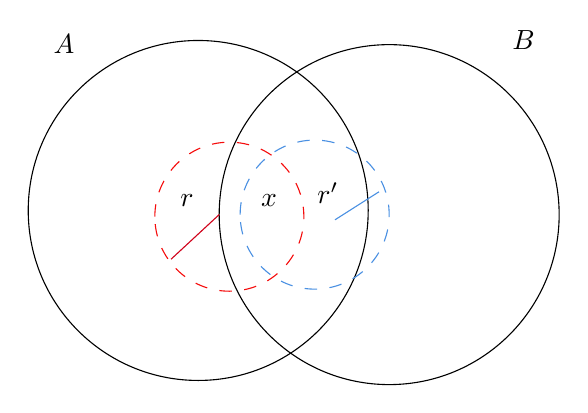
\begin{tikzpicture}[x=0.75pt,y=0.75pt,yscale=-1,xscale=1]
%uncomment if require: \path (0,300); %set diagram left start at 0, and has height of 300

%Shape: Circle [id:dp6379702365937482] 
\draw   (46,121.9) .. controls (46,76.67) and (82.67,40) .. (127.9,40) .. controls (173.13,40) and (209.8,76.67) .. (209.8,121.9) .. controls (209.8,167.13) and (173.13,203.8) .. (127.9,203.8) .. controls (82.67,203.8) and (46,167.13) .. (46,121.9) -- cycle ;
%Shape: Circle [id:dp3871343130648992] 
\draw   (138,123.9) .. controls (138,78.67) and (174.67,42) .. (219.9,42) .. controls (265.13,42) and (301.8,78.67) .. (301.8,123.9) .. controls (301.8,169.13) and (265.13,205.8) .. (219.9,205.8) .. controls (174.67,205.8) and (138,169.13) .. (138,123.9) -- cycle ;
%Shape: Circle [id:dp6625358626104291] 
\draw  [color={rgb, 255:red, 245; green, 12; blue, 12 }  ,draw opacity=1 ][dash pattern={on 4.5pt off 4.5pt}] (107,124.9) .. controls (107,105.07) and (123.07,89) .. (142.9,89) .. controls (162.73,89) and (178.8,105.07) .. (178.8,124.9) .. controls (178.8,144.73) and (162.73,160.8) .. (142.9,160.8) .. controls (123.07,160.8) and (107,144.73) .. (107,124.9) -- cycle ;
%Shape: Circle [id:dp6083087375414079] 
\draw  [color={rgb, 255:red, 74; green, 144; blue, 226 }  ,draw opacity=1 ][dash pattern={on 4.5pt off 4.5pt}] (148.1,123.9) .. controls (148.1,104.07) and (164.17,88) .. (184,88) .. controls (203.83,88) and (219.9,104.07) .. (219.9,123.9) .. controls (219.9,143.73) and (203.83,159.8) .. (184,159.8) .. controls (164.17,159.8) and (148.1,143.73) .. (148.1,123.9) -- cycle ;
%Straight Lines [id:da8851356973361522] 
\draw [color={rgb, 255:red, 208; green, 2; blue, 27 }  ,draw opacity=1 ]   (138,123.9) -- (114.8,145.4) ;
%Straight Lines [id:da800570752888615] 
\draw [color={rgb, 255:red, 74; green, 144; blue, 226 }  ,draw opacity=1 ]   (215,112.9) -- (193.8,126.4) ;

% Text Node
\draw (57,36.1) node [anchor=north west][inner sep=0.75pt]    {$A$};
% Text Node
\draw (278,34.1) node [anchor=north west][inner sep=0.75pt]    {$B$};
% Text Node
\draw (118,113.1) node [anchor=north west][inner sep=0.75pt]    {$r$};
% Text Node
\draw (184,107.1) node [anchor=north west][inner sep=0.75pt]    {$r'$};
% Text Node
\draw (157,113.1) node [anchor=north west][inner sep=0.75pt]    {$x$};


\end{tikzpicture}
    \end{center}
    
    $\implies$ Hagamos $r=min\{r,r'\}\implies$ si $y\in\mathbb{R}\ni d(x,y)<r\implies y\in A$ y $y\in B\implies y\in A\cap B\implies A\cap B$ es abierto en $\mathbb{R}^n$
    
\item \marginnote{$\bigcup_{i=1}^n A_i$.} Sea $\{G_\alpha\}$ una colección cualquiera de abiertos de $\mathbb{R}^n$ \marginnote{$\{G_\alpha:\alpha\in I\}$}, y sea $G=\bigcup_\alpha G_{\alpha} $. Si $x\in G\implies x\in G_\lambda$, para algún $\lambda$. Como $G_{\lambda}$ es abierto $\implies \exists r>0\ni B_r(x)\subset G_\lambda \subset $ 
    
\end{enumerate}
\end{proof}

\begin{remark}
La intersección de una colección infinita de abiertos, no necesariamente es abierta. En efecto, considere: $$A_n=\{x\in\mathbb{R}\ni -\frac{1}{n}<x<1+\frac{1}{n}\}, n\in\mathbb{Z}^+$$
$$A_1=(-1,2)$$
$$A_2=(-\frac{1}{2},\frac{3}{2})$$
\marginnote{Los $A_n$ son abiertos (por ser bolas abiertas en $\mathbb{R}$)}
$\implies A =\bigcap_{n=1}^\infty A_n=[0,1]$\footnote{¿Por qué cerrado?}
\end{remark}

\begin{definition}
Un subconjunto $\mathbb{F}$ en el métrico $(M,d)$ es cerrado si $\mathbb{F}^c$ es abierto. 
$[0,1]=(-\infty,0)\cup (1,\infty)\implies [0,1]$ es cerrado. 
\end{definition}

\begin{example}
\begin{enumerate}
    \item $\emptyset$ es abierto $\implies \emptyset^c=\mathbb{R}^n$ es cerrado. 
    \item $\mathbb{R}^n$ es abierto $\implies (\mathbb{R}^n)^c=\emptyset$ es cerrado. $\implies\emptyset$ y $\mathbb{R}^n$ son abiertos y cerrados. 
    \item $[0,1)$ no es abierto ni cerrado. 
    
\end{enumerate}
\end{example}